\chapter{Geo označevanje}
\label{ch:geo-oznacevanje}

Ste vedeli, da nekateri tviti vsebujejo oznako lokacije? Prav zares, nekateri imajo oznako geografske dolžine in širine, ki kaže na to, kje je bil tvit objavljen! Za konec tečaja si bomo pogledali, kako raziskati geolocirane tvite!

Z omrežja smo pridobili podatke za prvih nekaj dni leta 2017. Vsi tviti so bili objavljeni v Sloveniji, napisani pa so v različnih jezikih!

Prenesite slo-geo-tweets.tab z \url{http://file.biolab.si/text/slo-geo-tweets.tab} in poglejte podatke v gradniku \textit{Corpus Viewer}.

Ta korpus je precej poln informacij! Ne samo da imamo besedilo, število všečkov in čas objave, imamo tudi lokacijo in slike. Kakšno obilje informacij! Vsak tvit bomo prebrali posebej in…

\begin{marginfigure}[0cm]
    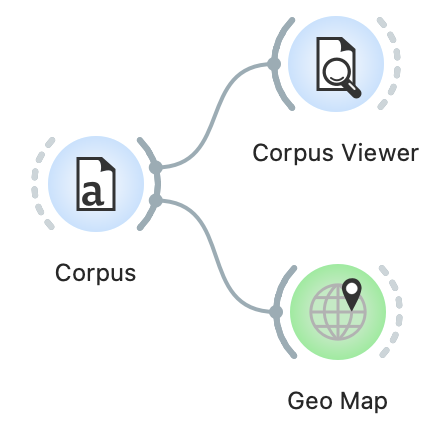
\includegraphics[width=\linewidth]{geo-workflow.png}
    \caption{}
\end{marginfigure}

Seveda ne bomo naredili tega! Do sedaj že vemo, da obstajajo hitrejši načini raziskovanja podatkov. Lahko jih na primer prikažemo na zemljevidu. Povežite Corpus z \textit{Geo Map} - gradnik bo avtomatsko našel stolpca latitude in longitude in prikazal podatke.

\begin{figure*}[h]
    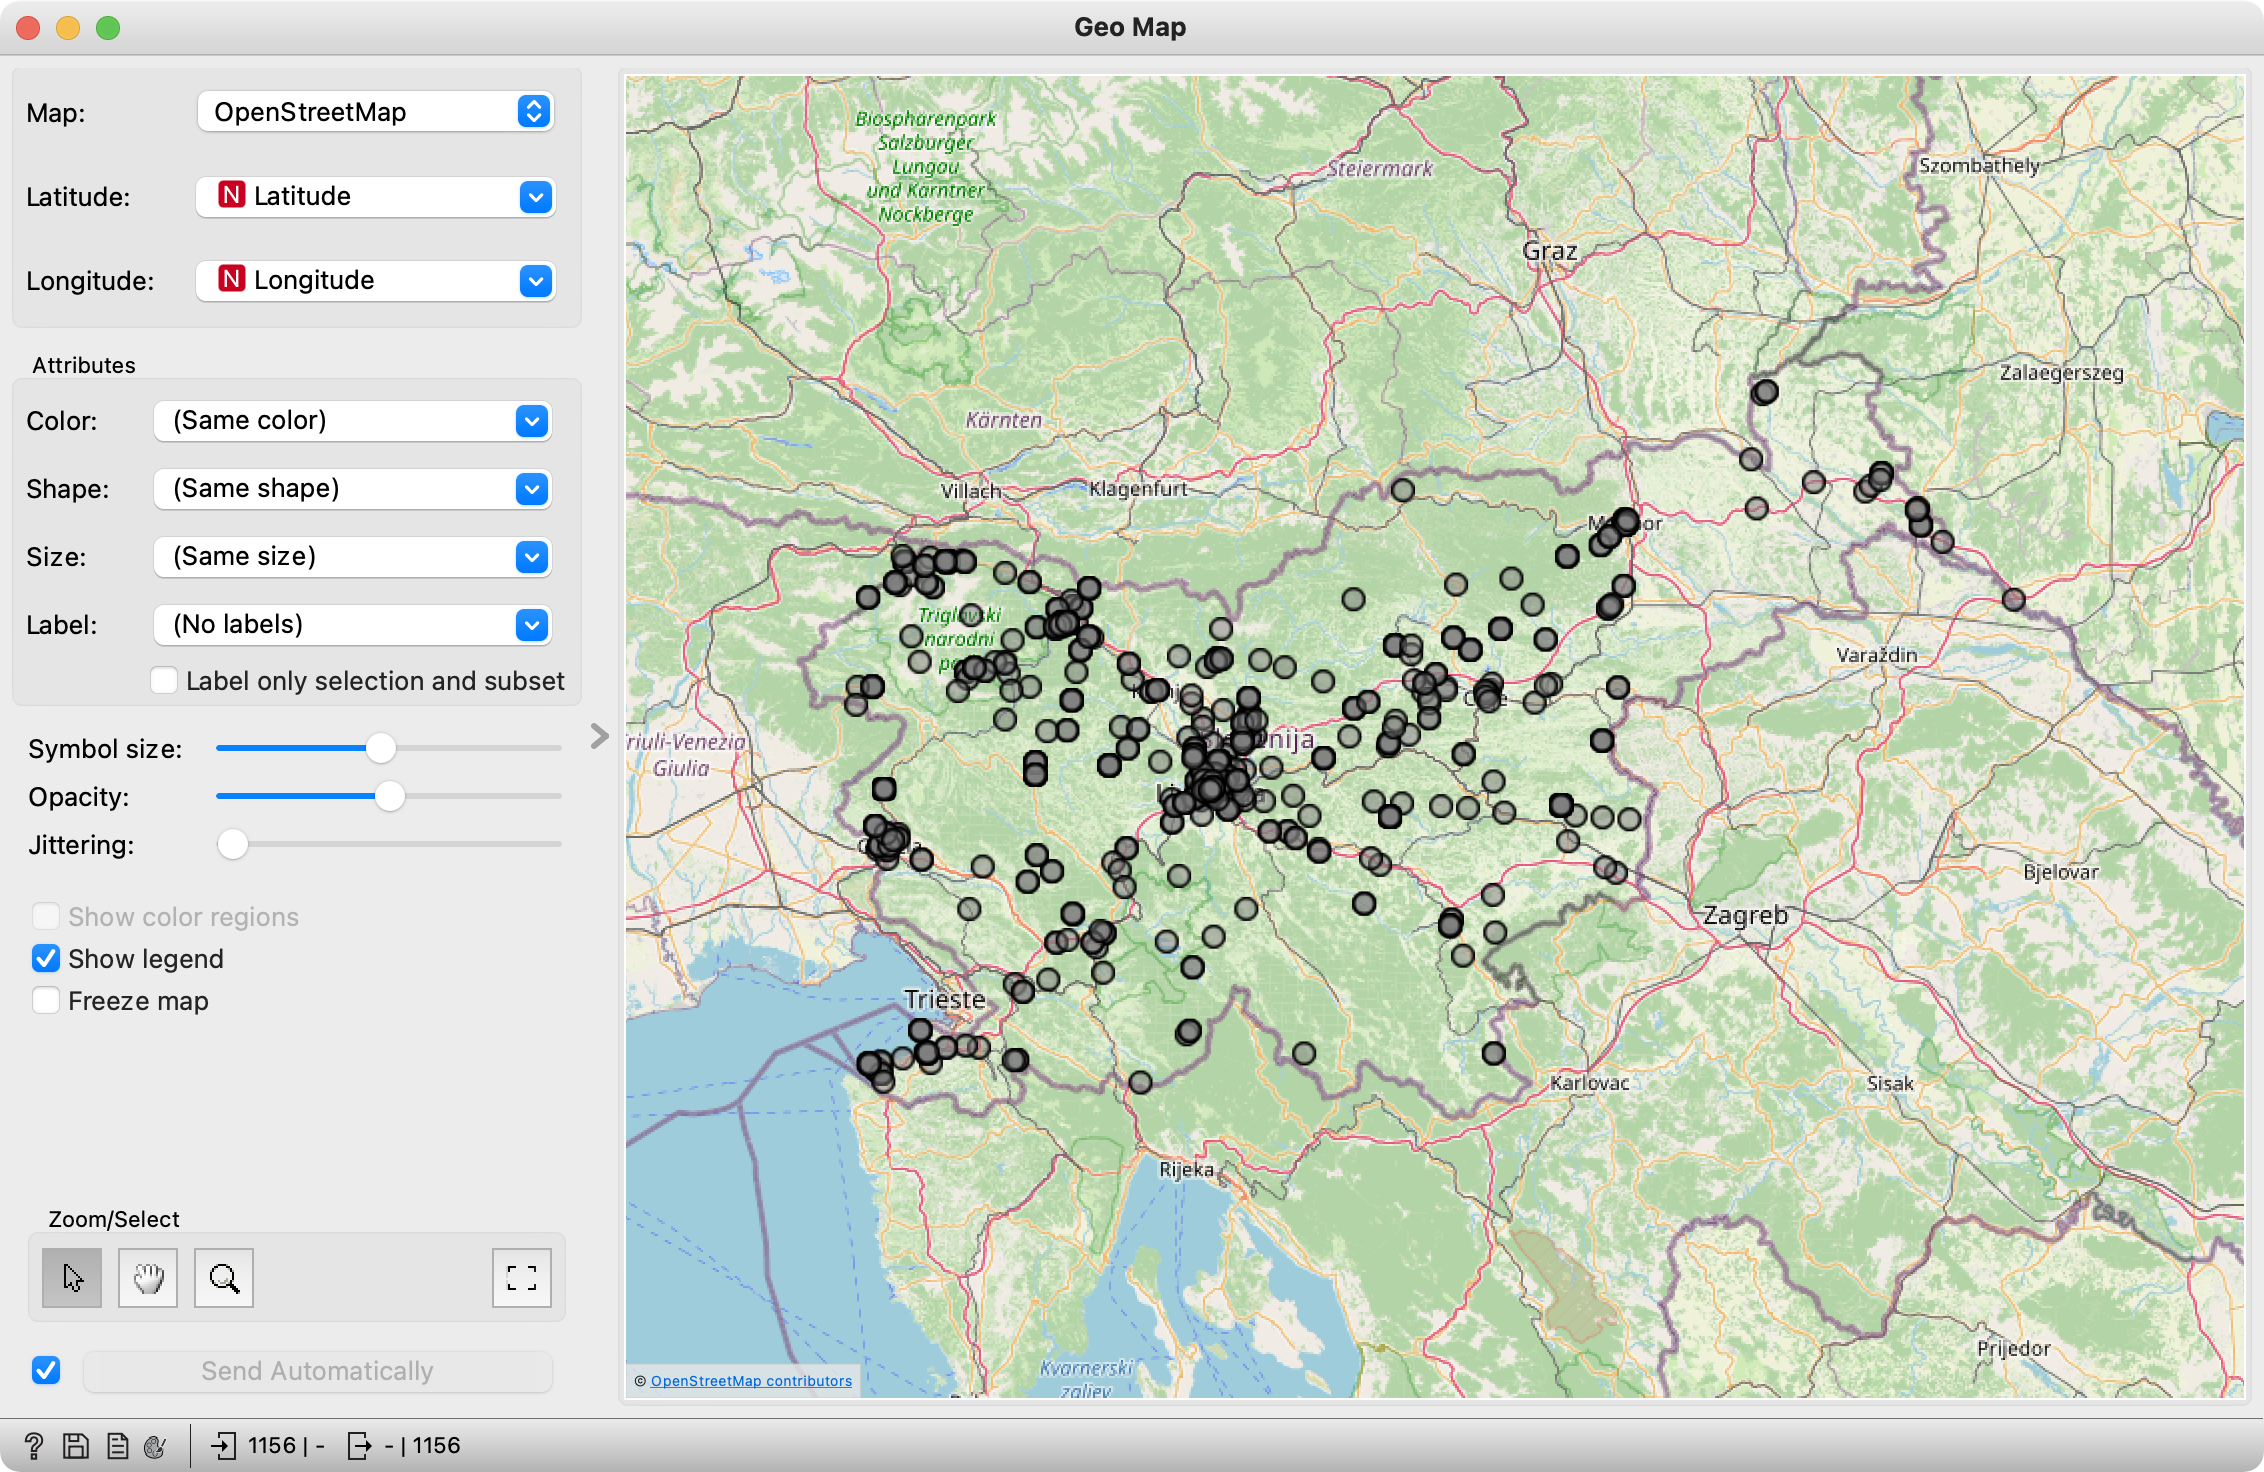
\includegraphics[width=\linewidth]{geo1.png}%
    \caption{}
    \label{fig:012-geo1}
  \end{figure*}

Dobro, sedaj vemo, da večina tvitov prihaja iz Slovenije in da so bolj pogosti v severo-zahodnem delu države.

Zanimiv podatek, ki smo ga pridobili, je, v katerem jeziku so bili tviti napisani. Ampak jezikov je ogromno! Zato moramo poenostaviti interpretacijo.

Corpus povežite z gradnikom \textit{Create Class}. Create Class ustvari novo spremenljivko iz obstoječih. Vrednosti bomo definirali v gradniku. Na primer, označiti želimo vse angleške tvite, zato bomo uporabili oznako ‘English’, če ima jezik vrednost ‘en’. Za slovenščino bomo uporabili ‘Slovenian’ za jezik ‘sl’ in tako naprej. Za vse druge jezike bomo uporabili oznako ‘foreign’.

Sedaj povežite Geo Map s Create Class. Naši geolocirani tviti bodo obarvani glede na jezik. To je že precej bolj zanimivo!

\begin{figure*}[h]
    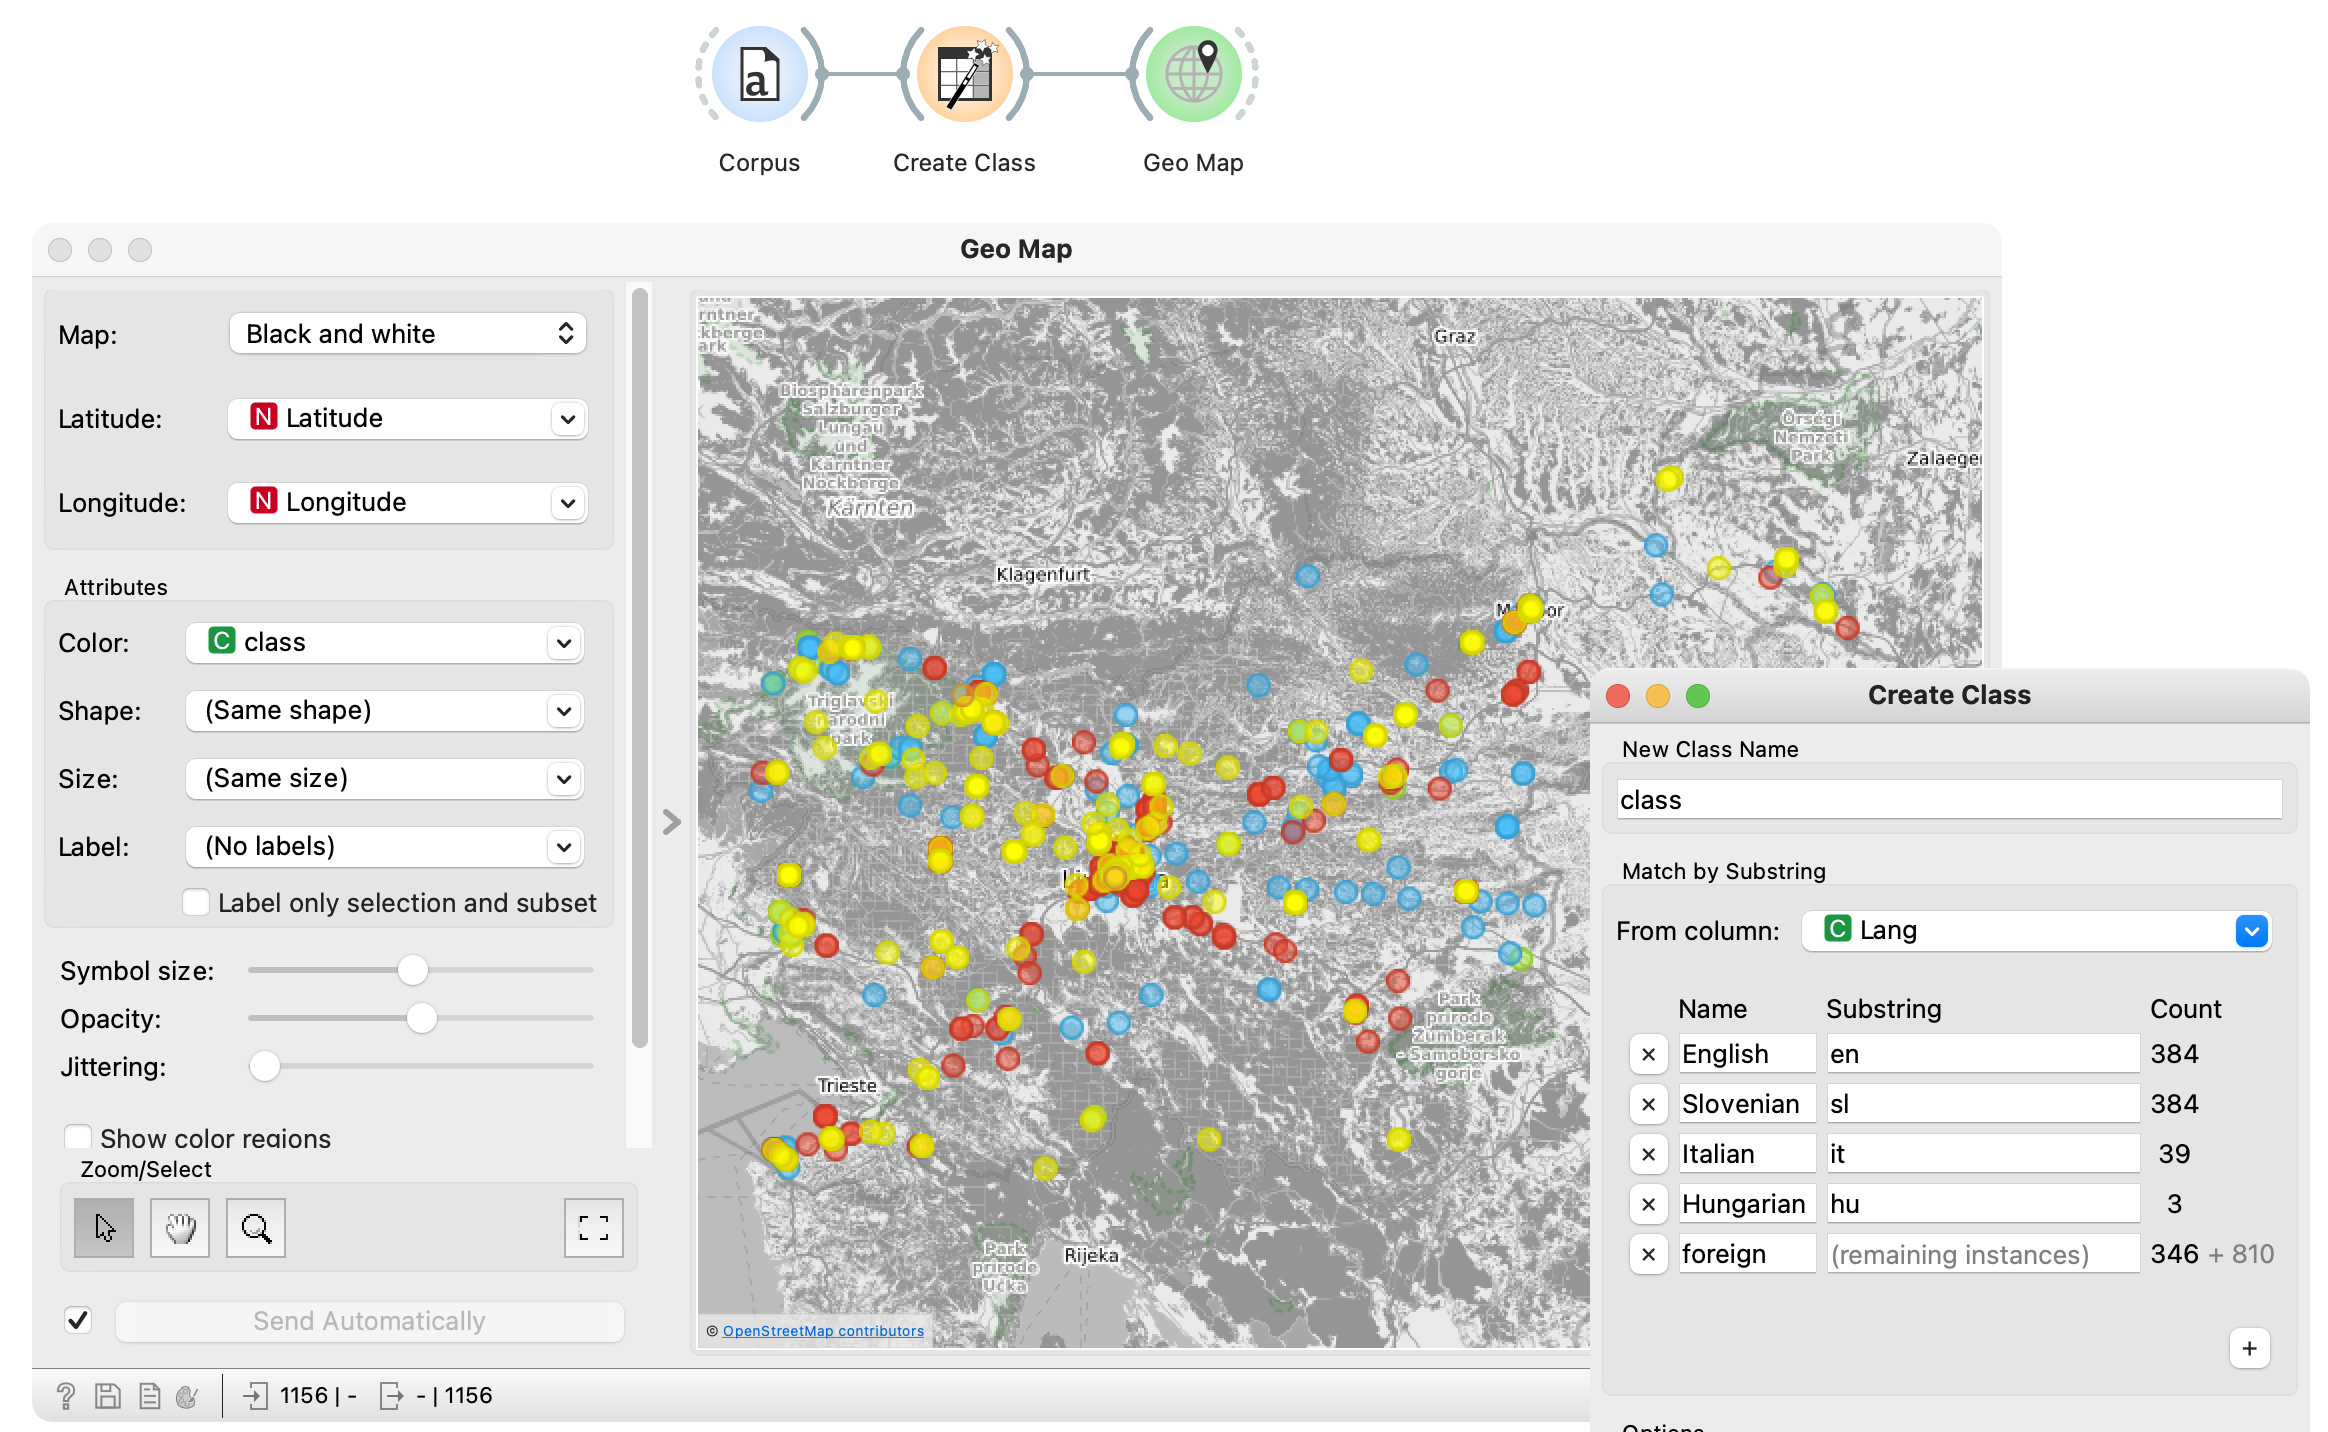
\includegraphics[width=\linewidth]{geo2.png}%
    \caption{}
    \label{fig:012-geo2}
\end{figure*}